% !TeX root = QuimNadalBargues_CV_Eng.tex
\documentclass[11pt,a4paper]{article}
\usepackage[utf8]{inputenc}
\usepackage[T1]{fontenc}
\usepackage[english]{babel}
\usepackage{graphicx}
\usepackage{tabularx}
\usepackage{hyperref}
\usepackage{multirow}
\usepackage{array}
\usepackage{ragged2e}
\usepackage{enumitem}
\usepackage{xcolor}
\usepackage{geometry}
\usepackage{fontawesome5} % Modern icon package

\geometry{a4paper, left=0.4in, right=0.4in, top=0.25in, bottom=0.25in}

\newcommand{\cvsection}[1]{
    \vspace{0.5em}
    \noindent\textbf{\large #1}
    \vspace{0.5em}
    \hrule\vspace{0.5em}
}
\newcommand{\cvsubsection}[1]{
\vspace{0.3em}
    \noindent\textbf{#1}
    \vspace{0.2em}
}

\newcommand{\skillsep}{\ {\color{gray}\textbar}\ }

\begin{document}

\noindent
\begin{minipage}{0.25\textwidth}
    \vspace*{10pt}
    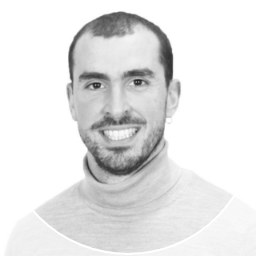
\includegraphics[width=\linewidth,keepaspectratio]{media/ProfilePicture.png} \\
    \cvsection{Contact}
    \begin{tabular}{@{}ll@{}}
        \faLinkedin & \href{https://www.linkedin.com/in/quimnadalbargues/}{Quim Nadal Bargués} \\
        \faHome & Barcelona, 22/04/1995 \\
        \faPhone & +34 620 200 817 \\
        \faEnvelope & \href{mailto:quimnaba@gmail.com}{quimnaba@gmail.com} \\
    \end{tabular}
    
    \cvsection{Languages}
        Spanish (Native) \\
        Catalan (Native) \\
        English (C1) \\
        
    \cvsection{Technical Skills}
        \begin{tabular}{@{}ll@{}}
        \textbf{Languages:}\\
          C\skillsep C++\skillsep Python\skillsep \\
          Bash\skillsep Java\skillsep VisualBasic\\
          XML\skillsep JSON\skillsep SQL\\
        \textbf{Control:}\\
          Matlab\skillsep Simulink \\
        \textbf{Embedded:}\\
            Lauterbach TRACE32\\ 
            J-Link (Segger)\\
        \textbf{Automotive:}\\
          Vector Tools\\
          ASPICE\skillsep Doors\\
        \textbf{Project Management:}\\
        Jira\skillsep Excel\skillsep SVN \\
        \textbf{General Software Skills:} \\
          Git\skillsep Windows\skillsep Linux\\
          CAN\skillsep ETH\skillsep RTP \\
          Android\skillsep Docker\skillsep LaTeX \\
          Enterprise Architect
          \end{tabular}
    
    
    \cvsection{Soft Skills}
    \begin{tabular}{@{}ll@{}}
        Humility            \\
        Work Cooperation    \\
        Decision-making     \\
        Logical thinking    \\
        Tolerance
    \end{tabular}
    
    \cvsection{Interests}
    \begin{tabular}{@{}ll@{}}
        Sports       \\
        Photography  \\
        Travel\\
        Driving Licenses: \\
        A, A2, A1, AM, B \\
    \end{tabular}
\end{minipage}
\hfill
\begin{minipage}[t]{0.68\textwidth} % Reduced from 0.72
    \vspace*{-26\baselineskip} % Pull content on top
    \nointerlineskip
    \begin{flushleft}
        {\fontsize{22}{0}\selectfont\bfseries Quim Nadal Bargués} \\ % Zero baselineskip
        \vspace{-8pt} % Pull rule up closer
        \rule{\linewidth}{0.5pt} \\
        \vspace{4pt}
        {\large\bfseries Telecommunications Engineer | Software Developer}
    \end{flushleft}
    
    % Professional Summary
    \cvsection{Professional Profile}
    Telecommunications engineer with 6+ years specializing in software electronic control systems, application software managing business logic, and embedded systems working with high-performance C++ and C applications. Proven track record in the whole development process: from software requirements definition, design, implementation, and validation.
    Experienced in international remote collaboration and performance optimization. \\
    
   
    \cvsection{Professional Experience}
    
    \noindent
    \textbf{Software Engineer} \hfill \textbf{Nov 2021 - Present} \\
    \textit{Creadis S.A | Wind Energy Sector} \hfill \textit{(Barcelona - Hybrid)} \vspace{4pt}
    
    Developed mission-critical electronic control applications for wind turbine software systems, for Vestas and Siemens Energy companies, going through all the development phases. All handling real-time data processing from 200+ sensors, its parameters, alarms... \\
    Key achievements include:
    \begin{itemize}[leftmargin=*,topsep=2pt,itemsep=-1pt]
        \item Redesigned lubrication subsystem using OOP principles, enabling coordinated control of dual pumps (funtionality and performance improvement)
        \item Developed an electronic control algorithm to compensate the faulty environmental sensors via discrete-time integration.
    \end{itemize}
    
    \vspace{10pt}
    
    \noindent
    \textbf{Software Engineer} \hfill \textbf{Feb 2018 - Nov 2021} \\
    \textit{Ficosa S.L | Automotive Sector} \hfill \textit{(Barcelona)} \vspace{4pt}
    
    Developed safety-critical C applications for Volkswagen Group's parking assistance systems.\\ Notable contributions:
    \begin{itemize}[leftmargin=*,topsep=2pt,itemsep=-1pt]
        \item Designed calibration application software algorithm (C) of a rear view camera meeting all functional requirements.
        \item Authored comprehensive software architectural documentation for the Rear View Camera system.
        \item Contributed to Top View Camera system design and requirements specification.
        \item Debugged complex field issues analyzing CAN, Ethernet and RTP traffic traces.
        \item Developed Python tool for automated Project Management (90\% faster milestone planning)
    \end{itemize}
    
    % Education with honors
    \cvsection{Education}
    \noindent
    \textbf{M.Sc. Computer Engineering} \hfill \textbf{2023 - Present (Expected 2026)} \\
    \textit{Universitat Oberta de Catalunya} \hfill \textit{Barcelona (Remote)} \\
    Specializing in Advanced Software Systems and Distributed Computing.\\
    Concurrent with full-time professional work.\\
    Relevant coursework: Cloud Architecture, Artificial Intelligence, Cibersecurity.\\
    \noindent
    \textbf{M.Sc. Telecommunications Engineering} \hfill \textbf{2013 - 2018} \\
    \textit{Universitat Politècnica de Catalunya} \hfill \textit{Barcelona}\\
    Specialized in Electronic Systems. Thesis on Ficosa's PM automation tool.\\    
\end{minipage}
\hspace{0.02\textwidth} % Added space between columns

\end{document}